\section{应用结果展示}  
%\label{chp:display}
在本节中,我们会对RunDroid运行结果做出相应的展示,并将展现结果和静态分析工具FlowDroid做对比,比较两个工具的产出结果,分析各自的优劣。

我们研究的APK的主体代码如\autoref{fig:code_demo}所示。
在\autoref{fig:code_demo}中,我们声明了有Activity\code{MainActivity},他是应用层的主Activity,该Activity界面主要有3个按钮组成,
方便对应的是斐波拉契数量的计算、启动一个Activity(生命周期相关)以及基于Handler的异步事件。



\begin{figure}[!h]
	\centering
	\vspace{0.7in}
	\begin{lstlisting}[language=Java]
package cn.mijack.rundroidtest;

public class MainActivity extends Activity implements View.OnClickListener {
	Button button1,button2,button3;
	Handler handler = new Handler() {
		public void handleMessage(Message msg) {
			if (msg.what == 1)    {
			      Toast.makeText(MainActivity.this, "handle", Toast.LENGTH_SHORT).show();
			}
		}
	};
	protected void onCreate(Bundle savedInstanceState) {
		super.onCreate(savedInstanceState);
		setContentView(R.layout.activity_main);
		button1 = findViewById(R.id.button1);
		button1.setOnClickListener(this);  
		// button2、button3进行相同的操作,此处省略
	}
	public void onClick(View view) {
		switch (view.getId()) {
			case R.id.button1:
				doHandleButton1();
				return;				
				// button2、button3进行相同的操作,此处省略
		}
	}
	public void doHandleButton1() {
		int fibonacci = doFibonacci(4);
		Toast.makeText(this, "fibonacci: " + fibonacci, Toast.LENGTH_SHORT).show();
	}
	private int doFibonacci(int i) {
		if (i < 1)			return -1;
		if (i == 1 || i == 2) 		return 1;
		return doFibonacci(i - 1) + doFibonacci(i - 2);
	}
	public void doHandleButton2() {
		Intent intent = new Intent(this, NewActivity.class);
		startActivity(intent);
	}
	public void doHandleButton3() {
		Thread workerThread =new WorkerThread(handler);
		workerThread.start();
	}
}\end{lstlisting}
	\caption{\question{待测试APK的主体代码}}
	\label{fig:code_demo}
\end{figure}



\subsection{函数调用图的构建结果展示}

在应用程序运行时,点击按钮button1,应用会计算斐波拉契数列中的第5项,并将这个数以Toast的形式展示给用户。
上述过程中,方法调用同时涉及到普通方法调用、递归函数调用。
RunDroid的动态分析结果如\autoref{fig:rundroid-result-Fibonacci}所示:
每一个红色节点对应的是一次方法执行,每一个绿色节点对应是一个对象;
如果对象是方法执行的方法对象,则在图中会有一条边从方法指向该对象,并在边上标识两种之间的关系(参数关系、返回值关系、实例关系等);
如果两个方法执行之间存在调用关系,则他们之间会通过从调用发起方指向被调用方的有向边进行连接。

在本案例中,\code{doHandleButton1()}调用了方法\code{doFibonacci()},因此前者有条有向边指向后者;
通过观察虚线框中各节点的关系,我们知道,对于方法\code{doFibonacci()},当参数为5时,对应的结果为5。
FlowDroid的静态分析结果如\autoref{fig:flowdroid-result-Fibonacci}所示。
通过比较\autoref{fig:rundroid-result-Fibonacci}和\autoref{fig:flowdroid-result-Fibonacci},我们可以发现以下有趣的结论:


\begin{figure*}[!ht]
	\centering
	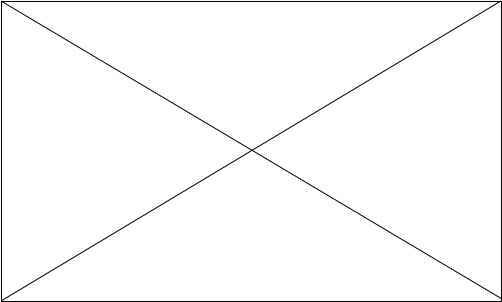
\includegraphics[width=\textwidth]{./Figures/empty.png}
	\caption{斐波拉契数列-RunDroid生成的调用图(局部)}
	\label{fig:rundroid-result-Fibonacci}
\end{figure*}

首先,两者在方法\code{doFibonacci()}数量上不同的:RunDroid得到的结果中,方法节点\code{doFibonacci()}共有9个,即在运行过程中,\code{doFibonacci()}被调用了9次。
由于在一个应用中,一个方法的方法签名是唯一的,所以FlowDroid给出的结果中\code{doFibonacci()}只有一个节点,该节点上存在一个指向自己的环,表示这个方法在执行过程中可能出现递归调用的情况。
另外,静态分析方法(FlowDroid)在分析\code{doFibonacci()}这类方法时,对函数的执行上下文做出准确的判断,进而给出程序准确的运行时行为。
因此,静态分析技术得到的函数调用图往往以方法体本身作为研究的基本单元,而动态分析技术的函数调用图可以细化方法执行之间的关系,在一定程度上可以反映程序执行的具体过程。



其次,方法\code{Toast.makeText(Context,CharSequence,int)}没有出现在RunDroid的结果中,而FlowDroid给出的结果却有展现:
而在运行过程中,我们却可以看到Toast提示。
经过分析,原因如下:\code{Toast.makeText(Context,CharSequence,int)}属于系统定义的方法,而运行时拦截器待拦截的方法列表中并未包含该方法,因此运行时未收集到相关的方法执行信息,导致RunDroid无法在调用图中还原相应的函数。
这也从一个方面反映了RunDroid的劣势:系统函数运行时信息的捕获需要提前将相应的方法告知运行时拦截器,生成的调用图才会包括相应的方法。
这使得调用图只包含研究人员关心的方法的执行信息,但也在一定程度上导致部分方法的缺失和调用图的局部不完整。


\begin{figure*}[!ht]
	\centering
	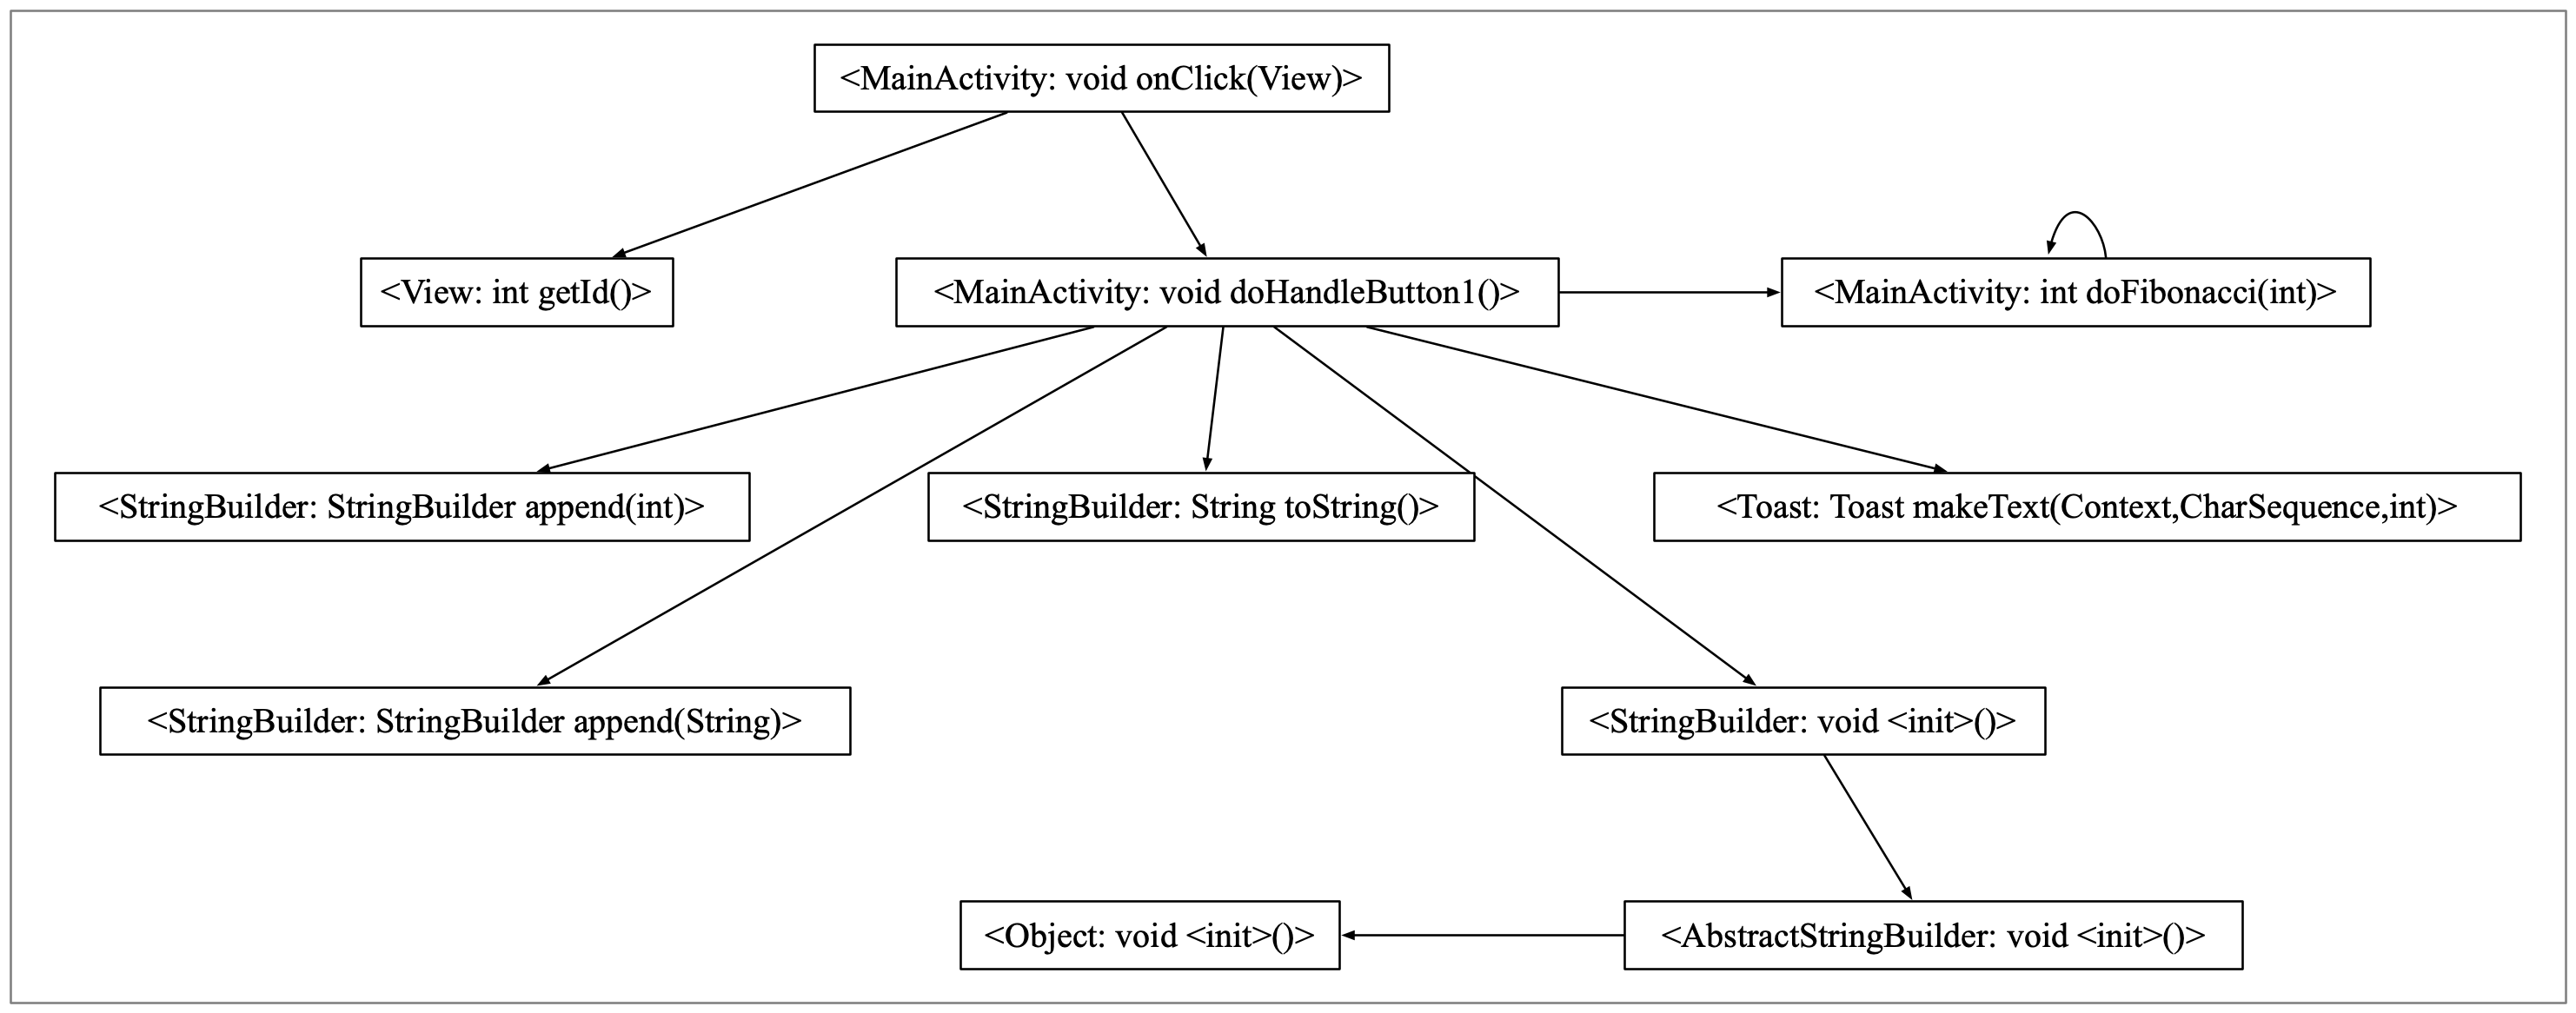
\includegraphics[width=\textwidth]{./Figures/FlowDroid-Fibonacci.png}
	\caption{斐波拉契数列-FlowDroid生成的调用图(局部)}
	\label{fig:flowdroid-result-Fibonacci}
\end{figure*}


最后,FlowDroid给出的结果中包括了大量和\code{StringBuilder}相关的方法,而RunDroid的结果并不包括这些方法:
对比源码发现,源程序并未直接使用\code{StringBuilder}。
通过查阅文献\cite{gosling2000java},我们发现出于提高字符串串联性能的考虑,Java编译器可以使用类\code{StringBuilder}等技术通过源代码做适当等价的修改,以避免表达式求值过程中产生过多的字符串数量。
由于上述过程发生在Java程序编译阶段并最后以字节码的形式不存在APK文件中,而FlowDroid恰好从字节码层面对应用进行分析,因此FlowDroid的分析结果会包含该方法。
对于RunDroid,上述方法既在源代码中未出现相关方法定义(无法进行日志代码编织),又不在运行时拦截器的目标方法列表中,所以RunDroid给出的调用图自然也不会包括\code{StringBuilder}相关的方法。



\subsection{Activity 生命周期和事件回调的效果展示}

在本节中,应用运行时,我们将点击按钮button2,在\code{MainActivity}启动另一个\code{NewActivity},对比RunDroid和FlowDroid在Activity生命周期方法的呈现效果。
最终,我们得到的RunDroid的运行结果如\autoref{fig:rundroid-result-lifecycle}所示。
针对Android 组件\code{Activity}的生命周期特性,FlowDroid 进行了针对性的建模,通过构造方法\code{dummyMainMethod()}串联Android Activity的生命周期和UI事件回调,相应的结果如\autoref{fig:flowdroid-result-lifecycle}所示。

\begin{figure*}[ht]
	\centering
	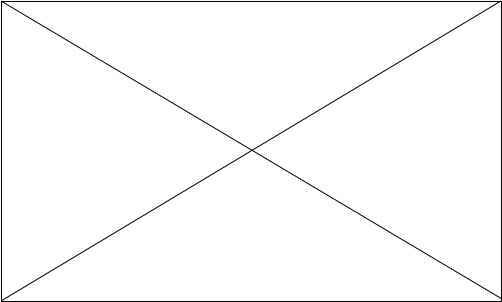
\includegraphics[width=\textwidth]{./Figures/empty.png}
	\caption{Activity部分-RunDroid生成的调用图(局部)}
	\label{fig:rundroid-result-lifecycle}
\end{figure*}

对比\autoref{fig:rundroid-result-lifecycle}和\autoref{fig:flowdroid-result-lifecycle},
我们可以发现RunDroid和FlowDroid在组件生命周期和事件回调上的设计思想上是不同的:
RunDroid可以捕获到组件生命周期方法以及回调事件方法的实际执行,因此,RunDroid对于上述行为的展现主要是按照时间的先后顺序将这些方法节点串联起来,形成完整的事件序列。
而FlowDroid在生成函数\code{dummyMainMethod()}时,会为AndroidManifest.xml文件中定义的每一个Activity单独创建包含生命周期方法和事件回调方法的状态迁移图
(\autoref{fig:flowdroid-result-lifecycle}中的虚线框部分表示Activity的整体状态迁移,灰色部分为\code{MainActivity}中的UI事件响应方法),
最后将这些Activity的状态迁移串联起来,并将Action为\code{android.intent.action.MAIN}并且category为\code{android.intent.category.LAUNCHER}的Activity组件作为结果的默认启动的Activity,最终形成方法\code{dummyMainMethod()}。


\begin{figure*}[ht]
	\centering
	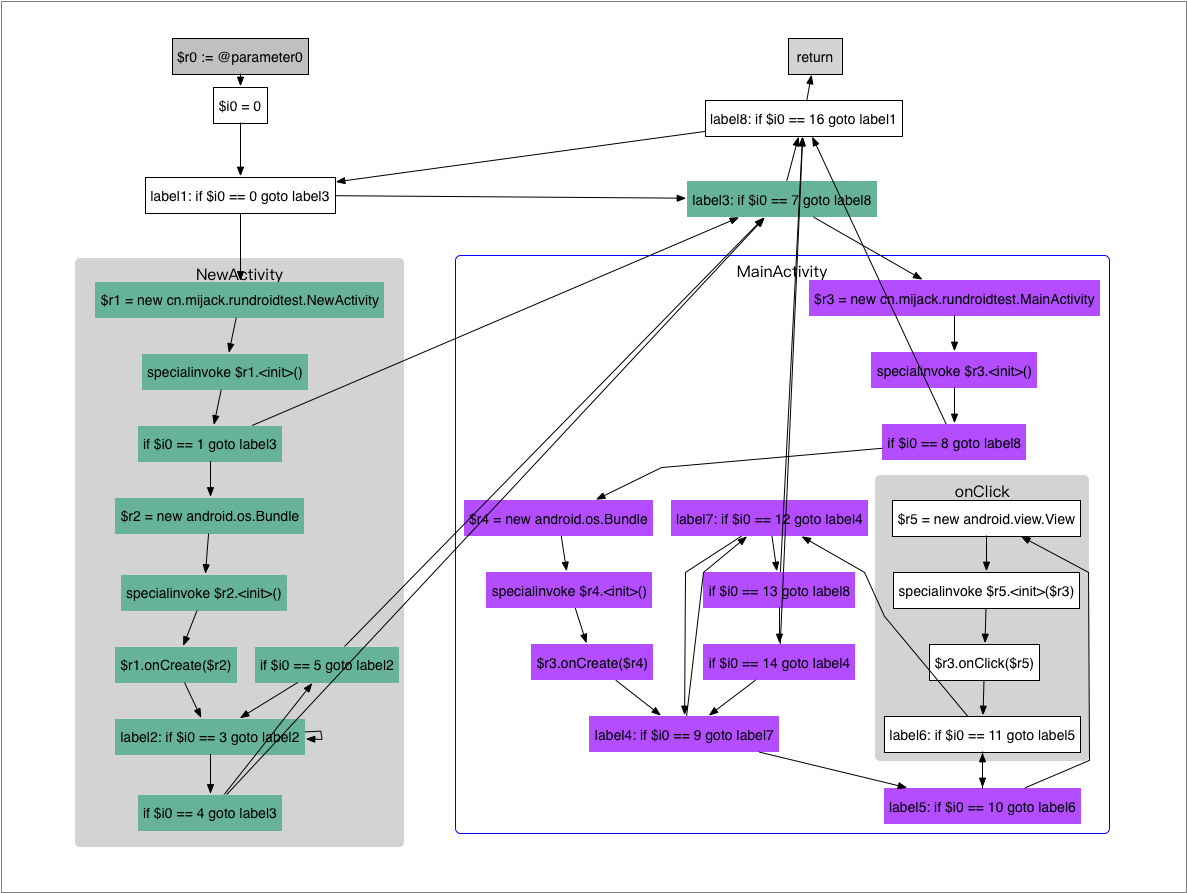
\includegraphics[width=\textwidth]{./Figures/flowdroid-dummyMainMethod.png}
	\caption{dummyMainMethod-FlowDroid生成的调用图}
	\label{fig:flowdroid-result-lifecycle}
\end{figure*}

在结果展现上,RunDroid倾向于将和Activity生命周期相关的所有方法都关联起来。
例如,虽然开发人员在源代码中没有定义\code{onResume()}等方法,但在运行过程中,\code{MainActivity}的父类方法\code{onResume()}被调用了,便会在结果中呈现出来。
在这点上,FlowDroid的处理方式恰恰相反,考虑到在未重写系统类方法时的类行为表现基本保持一致性,FlowDroid并不会在结果中展示父类Activity未重载的生命周期方法。


\question{观察\autoref{fig:rundroid-result-lifecycle}中生命周期方法归属的Activity,我们发现,在应用启动\code{NewActivity}过程中,
\code{MainActivity}和\code{NewActivity}的生命周期方法是交替出现的,并不是\code{MainActivity}的生命周期方法全部执行完毕后才执行\code{NewActivity}的生命周期方法。
而FlowDroid给出的结果将\code{MainActivty}和\code{NewActivity}分开处理,因此得到的结果属于后面一种情况。
相比FlowDroid,RunDroid的运行结果是程序运行时的直接反映,更适合反映应用的状态变化。
}

\subsection{多线程触发关系效果展示}

多线程开发是Android开发中经常涉及的开发要求。
为此,针对这一场景,我们进行了相关的测试。
在本节,我们将点击按钮button3,获取\code{doHandleButton3()}相关的调用图情况。
经过实验,RunDroid和FlowDroid的运行结果分别如\autoref{fig:rundroid-result-handler}、\autoref{fig:flowdroid-result-handler}所示。
两幅图在以下节点上存在不同:





\begin{figure*}[ht]
	\centering
	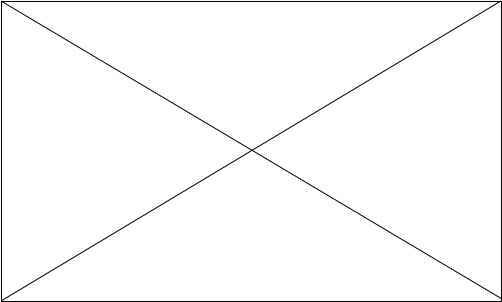
\includegraphics[width=\textwidth]{./Figures/empty.png}
	\caption{多线程触发关系-RunDroid生成的调用图(局部)}
	\label{fig:rundroid-result-handler}
\end{figure*}




\begin{figure*}[ht]
	\centering
	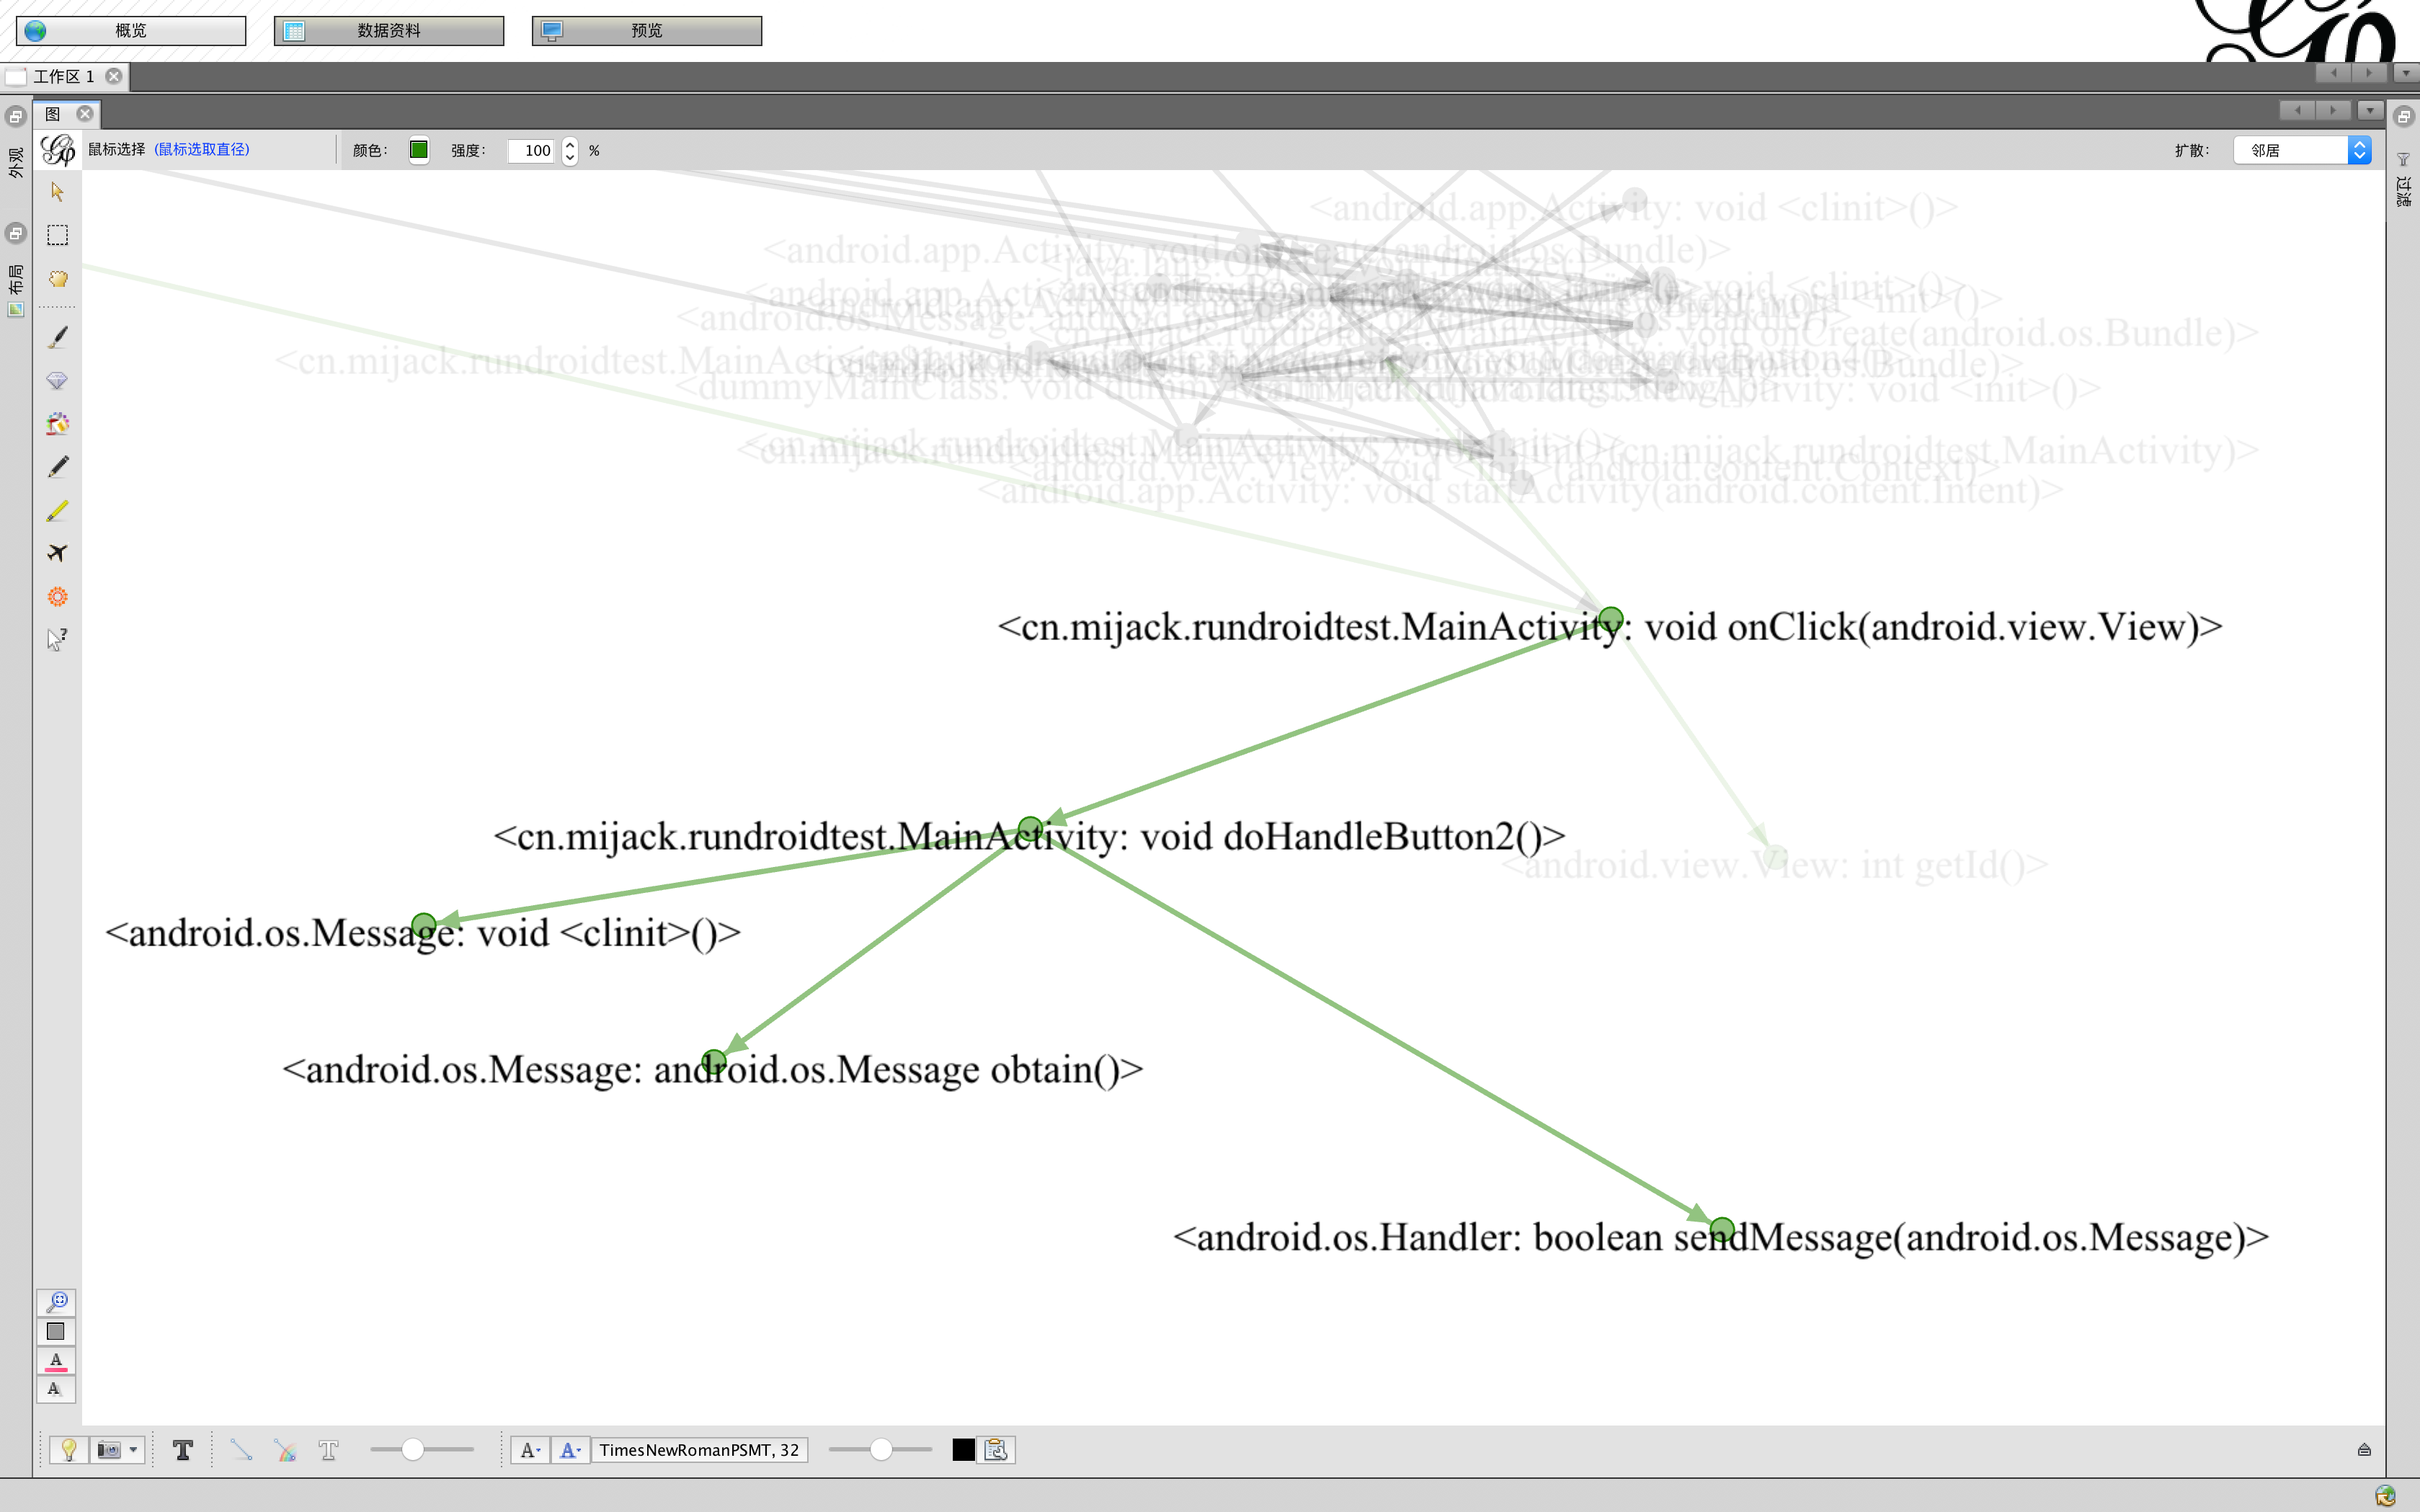
\includegraphics[width=\textwidth]{./Figures/FlowDroid-handler.png}
	\caption{多线程触发关系-FlowDroid生成的调用图(局部)}
	\label{fig:flowdroid-result-handler}
\end{figure*}


\point{Java API多线程的触发方式}

RunDroid在方法\code{Thread.start()}和方法\code{WorkerThread.run()}之间添加了一条有向边。
这条有向边从前者指向后者,表示方法\code{Thread.start()}的执行触发了方法\code{WorkerThread.run()}的执行,边上标识着触发原因(通过Thread方式触发,Thread)。
FlowDroid对方法\code{doHandleButton3()}进行推算出\autoref{fig:code_demo}第42行中的变量$workerThread$类型为\code{WorkerThread}。
同时,FlowDroid可以推算出方法\code{Thread.start()}的执行会导致方法\code{WorkerThread.run()}的执行。
在FlowDroid的设计者看来,方法\code{Thread.start()}可以替换成方法\code{WorkerThread.run()}。
因此,FlowDroid的结果中,方法\code{doHandleButton3()}和\code{WorkerThread.run()}之间存在调用边。
这条有向边并不是像RunDroid从\code{Thread.start()}出发。
虽然RunDroid和FlowDroid都可以在函数调用图表现Java API多线程的触发方式,但相比之下,RunDroid的呈现方式更为全面严谨,比FlowDroid更符合程序的运行过程。
当方法\code{Thread.start()}和\code{WorkerThread.run()}同时在同一个函数中被调用,FlowDroid在调用图上无法将这两个方法间的调用关系和触发关系区分开。
而RunDroid针对性地标识了函数间的关系是普通调用关系还是基于线程的触发关系,所以不会在方法关系展现上遇到类似的问题。


\point{基于Handler的多线程触发方式}

在WorkerThread的方法run()中,我们通过Handler进行了异步UI操作,触发了方法\code{MainActivity\$1.handleMessage(Message)}的执行。
在构建拓展调用图过程中,RunDroid充分挖掘了这些方法和对应的方法对象的关联关系,进而补全方法\code{Handler.sendMessage()}和\code{MainActivity\$1.handleMessage(Message)}之间的触发关系。
因此,在RunDroid展示的结果中,上述两个方法之间存在一个从前者指向后者的有向边,边上标识着相应的触发原因(通过Handler方式触发,Handler)\footnote{由于我们定义的Handler是MainActivity的匿名内部类,因此,编译后的类名为\code{MainActivity\$1}}。
但是,FlowDroid分析相关代码时,由于缺少运行时上下文的基本信息,无法分析出\code{WorkerThread.run()}中handler的具体类型,因此,无法将Handler相关的两个方法连接起来。




\point{静态方法的使用}


另外,在FlowDroid给出的结果中,我们发现方法\code{doHandleButton3()}还调用了类\code{Message}的类初始化方法\code{<clinit>()}。
原因是方法\code{doHandleButton3()}调用类\code{Message}的静态方法\code{obtain()},因此可能需要进行类的初始化。
由于在程序运行过中,方法\code{doHandleButton3()}在执行方法\code{Message.obtain()}前,类\code{Message}已经完成了类的初始化,方法\code{Message.<clinit>()}并没有被调用。
因此RunDroid的结果中显示上述两个方法不存在调用关系。
这从一个侧面方面反映出FlowDroid分析的结果和动态运行的过程可能存在一定的偏差。



%\section{RunDroid和FlowDroid的对比总结}

\section{本章小结}

% 本章中,我们将环绕着构建效率、日志效率、运行效率等三个方面对RunDroid角进行系统性能测试和评估,并结合实验结果阐述了采用源代码插桩、基于MMap的日志方案等原因。
 
本章结合具体的使用场景对RunDroid生成的拓展函数调用图做了较为详细的描述。
同时,我们还对比分析在相同场景下静态分析工具FlowDroid的运行结果。
我们发现,RunDroid生成的调用图的完整性依赖于源代码处理以及待拦截的目标系统方法列表的完整程度,而FlowDroid的分析对象是Android应用程序APK文件,调用图的完整性受到自身算法实现的限制。
另外,两者在设计思想上不同的,RunDroid关心的是在程序执行过程中的方法之间的依赖关系,而FlowDroid反映的是从函数执行角度两个方法(包括递归调用)之间是否存在调用的可能性。
前者是某一应用运行的具体、微观的表现,而后者更多的是反映方法调用关系在宏观、理论上的可能性。
综上,RunDroid和FlowDroid体现方法的调用关系上各有千秋。

